\documentclass{standalone}
\usepackage{tikz}
\usepackage{color}
\usetikzlibrary{positioning, shapes, arrows.meta, calc, decorations.pathreplacing}

\definecolor{myblue}{RGB}{82,126,171}
\definecolor{myred}{RGB}{168, 50, 50}

\tikzset{
  square/.style={draw,outer sep=5,inner sep=1,minimum size=10,line width=0, 
    very thick, draw=myblue, top color=white,bottom color=white}, 
  noborder/.style={draw,outer sep=0,inner sep=0,minimum size=20,line width=1, 
    draw=none, scale=1, anchor=west},
  blue/.style={draw,outer sep=35,inner sep=3,minimum size=20, line width=1, 
    very thick, draw=none, top color=myblue, bottom color=myblue, scale=1.25},
   noborderr/.style={draw,outer sep=0,inner sep=0,minimum size=20,line width=1, 
    draw=none, scale=1, anchor=west}
}

\begin{document}

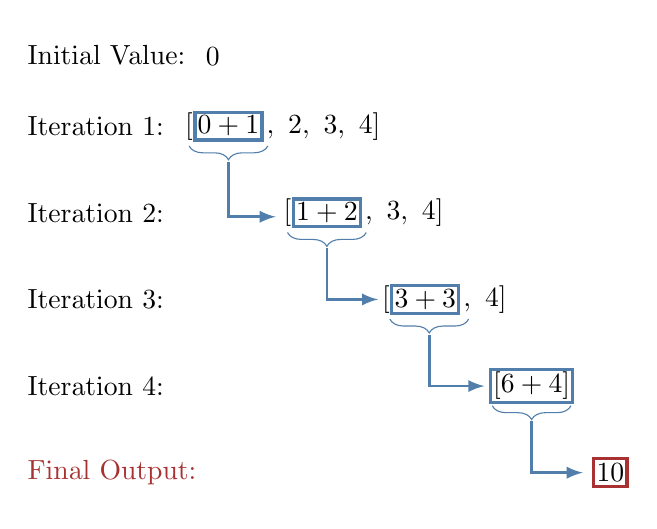
\begin{tikzpicture}

\draw[decorate,color=myblue,decoration={brace,amplitude=5pt}] (-1.2,2.55) -- (-2.2,2.55);
\draw[-latex,line width=1 pt,color=myblue] (-1.7,2.35) |- (-1.1,1.65);


\node [noborderr] at (-2.25,3.68) {$0$};


%\node [noborderr] at (-2.25,2.8) {$[ 0+1, ~2, ~3,~ 4]$};
\node [noborderr] at (-2.25,2.8) {$[ ~~~~~~~~, ~2, ~3,~ 4]$};
\node [square] at (-1.7,2.8) {$0 + 1$};


\draw[decorate,color=myblue,decoration={brace,amplitude=5pt}] (0.05,1.45) -- (-0.95,1.45);
\draw[-latex,line width=1 pt,color=myblue] (-0.45,1.25) |- (0.2,0.6);

\node [noborderr] at (-1,1.7) {$[ ~~~~~~~~, ~3,~ 4]$};
\node [square] at (-0.45,1.7) {$1 + 2$};


\draw[decorate,color=myblue,decoration={brace,amplitude=5pt}] (1.35,0.35) -- (0.35,0.35);
\draw[-latex,line width=1 pt, color=myblue] (0.85,0.15) |- (1.55,-0.5);

\node [noborderr] at (0.25,0.6) {$[ ~~~~~~~~,~ 4]$};
\node [square] at (0.8,0.6) {$3+ 3$};


\draw[decorate,color=myblue,decoration={brace,amplitude=5pt}] (2.65,-0.75) -- (1.65,-0.75);
\draw[-latex,line width=1 pt,color=myblue] (2.15,-0.95) |- (2.8,-1.6);

\node [square] at (2.15,-0.5) {$[6 + 4]$};
\node [square,draw=myred] at (3.15,-1.6) {$10$};


\node [noborderr] at (-4.25,3.7) {Initial Value:};
\node [noborderr] at (-4.25,2.8) {Iteration 1:};
\node [noborderr] at (-4.25,1.7) {Iteration 2:};
\node [noborderr] at (-4.25,0.6) {Iteration 3:};
\node [noborderr] at (-4.25,-0.5) {Iteration 4:};
\node [noborderr, color=myred] at (-4.25,-1.6) {Final Output:};


\end{tikzpicture}

\end{document}
